%\documentclass[12pt]{article}
%\usepackage[a4paper, margin=1in]{geometry} 
%\usepackage{graphicx} 
%\usepackage{hyperref}
%\usepackage{float}
%\usepackage{multicol}
%\usepackage{multirow}
%\usepackage{amsmath}
%\usepackage[ruled]{algorithm2e}
%\usepackage[font=small, labelfont=bf]{caption}
%
%\begin{document}

%
% Maximum likelihood
%
\subsection{Maximum likelihood}
The maximum likelihood can be used to reconstruct a phylogenetic tree.

%
%  Conditinal probabilities
%
\subsubsection*{Conditinal probabilities}
\begin{itemize}
\item $P(H|D)$ where $D$ is observed data and $H$ is a hypothesis
\item $P(M|D)$ where $D$ is observed data and $M$ is a model
\end{itemize}

\noindent
Not easy to sovle $P(H|D)$ or$ P(M|D)$ directly

%
%  Bayes' theorem
%
\subsubsection*{Bayes' theorem}
\medskip 

\[
P(H|D) = \dfrac{P(D|H)P(H)}{P(D)}
\]

\begin{itemize}
\item $P(H|D)$, $P(M|D)$: conditinal probabilities
\item $P(H)$, $P(D)$: maginal probabilities
\item $P(H|D)$: posterior probability
\item $P(H)$: prior probability
\item $P(D|H)$: likelyhood
\item $L(H|D)$: likelyhood function (equivalent with $P(D|H)$)
\end{itemize}

%
%  Maximum likelihood
%
\subsubsection*{Maximum likelihood}
We assume a uniform prior distribution for $P(H)$. Then, we can find the hypothesis that achieves the maximum likelyhood $L(H|D)$. \\


${\displaystyle {\hat {\theta }}\in \{{\underset {\theta \in \Theta }{\operatorname {arg\,max} }}\ L(\theta|D)\}}$

%
%  Example of maximum likehood
%
\subsubsection*{Example of fair and unfair dice}
Roll a die three times, and a 6 comes up three times in a row.

\begin{figure}[H]
  \centering
      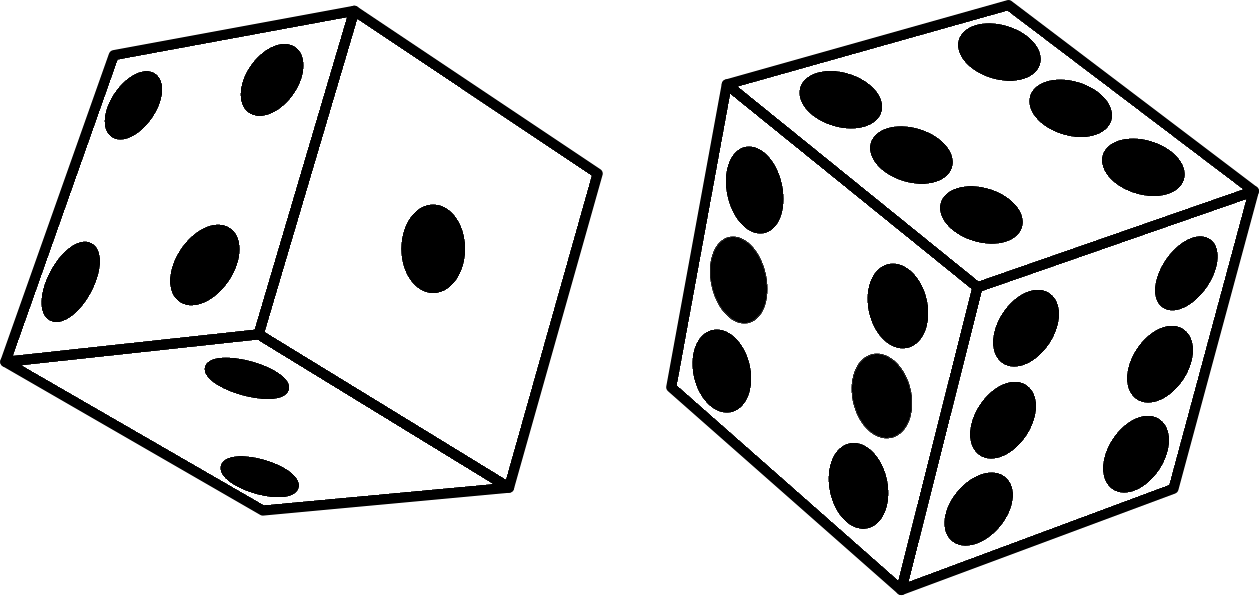
\includegraphics[width=0.3 \textwidth]{fig09/dice_unfair.png}
        \caption{Two dice - a fair die and a die with three 6’s}
\end{figure}

\noindent
Probabilities:
\begin{itemize}
\item Three die roles with a fair die $P(D|H = fair) = (1/6)^3 \simeq 0.028$
\item Three die roles with the unfair die: $P(D|H = unfair) =(3/6)^3 = 0.125$
\end{itemize}

\noindent
Maximum likelihood:
\begin{itemize}
\item ${\displaystyle {\underset {\theta \in (fair, unfair) }{\operatorname {arg\,max} }}\ L(\theta|D)} = unfair$
\end{itemize}

%
%  Tree search method of maximum likelihood
%
\subsubsection*{Tree search method of maximum likelihood}
The maximum likelihood method is also based on tree search. It tries to find the tree with the hightest likelihood for a given MSA.

%
%  Example of tree search method 
%
\subsubsection*{Example of tree search method }
Calculate the likelihood $L(T=tree1|D )$.
 
 \begin{figure}[H]
  \centering
      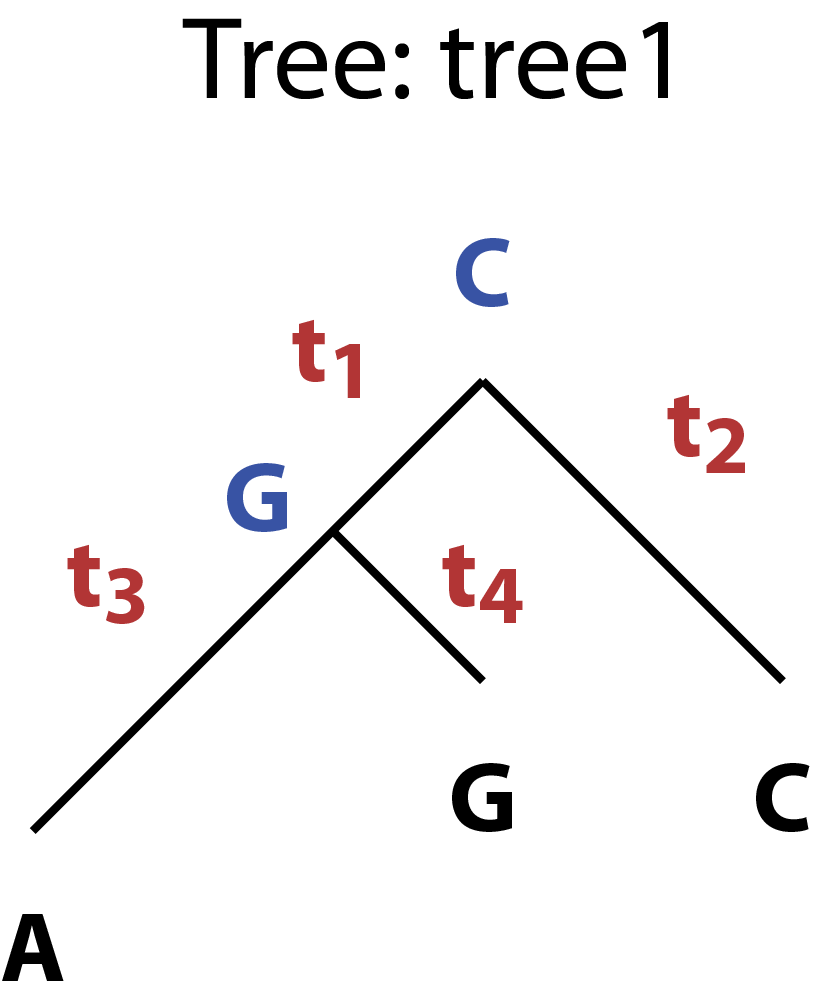
\includegraphics[width=0.2 \textwidth]{fig09/ml_tree.png}
      \caption{Two dice - a fair die and a die with three 6’s}
\end{figure}
 
Likelihood: $L(T=tree1|D ) = P(D|T=tree1 )=P_{CG}(t{1})P_{CC}(t_{2})P_{GA}(t_{3})P_{GG}(t_{4})$

%
% Log-likelihood
%
\subsubsection*{Log-likelihood}
\begin{itemize}
\item Logarithm is a monotonically increasing function 
\item $\log⁡(ab)=\log⁡(a)+\log⁡(b)$
\end{itemize}

%
% Time complexity of tree search
%
\subsubsection*{Time complexity of tree search}
Since it needs to search all possible trees, both the maximum parsimony and the maximum likelihood methods are NP hard problems. 
\begin{itemize}
\item Exhaustive search: up to 8-10 sequences
\item Branch and bound or pruning: up to 15-20 sequences
\item Heuristics: 100+ sequences
\end{itemize}

\bigskip 

%\end{document}
